\documentclass[a4paper,14pt]{extarticle} \usepackage[utf8]{inputenc}
\usepackage[T1]{fontenc}
\usepackage[margin=2.5cm]{geometry}

% Fonte Caladea se existir, senão lmodern
\IfFileExists{caladea.sty}{
  \usepackage{caladea}
}{
  \usepackage{lmodern} }
\usepackage{ragged2e}
\usepackage{graphicx}
\usepackage[portuguese]{babel}
\usepackage{wrapfig}
\usepackage{hyperref}
\usepackage{fancyhdr}
\usepackage{xcolor}
\usepackage{rotating}
\usepackage{titlesec}
\usepackage{epigraph}
\usepackage{dirtytalk}
\usepackage{indentfirst} % Indenta o primeiro parágrafo após seções

% Ajuste do recuo de parágrafo
\setlength{\parindent}{1.5em}

% Centralizar títulos
\titleformat{\section}
  {\normalfont\centering\bfseries\Large}{\thesection}{1em}{}

\titleformat{\subsection}
  {\normalfont\centering\bfseries\large}{\thesubsection}{1em}{}

\titleformat{\subsubsection}
  {\normalfont\centering\bfseries}{\thesubsubsection}{1em}{}

% -------------- Símbolos de Versículo e Resposta --------------
% Definição do símbolo (a “barrinha” inclinada)
\makeatletter
\newcommand{\vers@resp@sym}{%
  \raisebox{0.2ex}{\rotatebox[origin=c]{-20}{$\m@th\rceil$}}%
}
% macro interna que sobrepõe a barrinha e a letra V ou R
\newcommand{\vers@resp}[2]{%
  {\ooalign{%
     \hidewidth\kern#1\vers@resp@sym\hidewidth\cr
     #2\cr
  }}%
}
% comandos públicos \versicle e \response
\DeclareRobustCommand{\versicle}{\vers@resp{-0.1em}{V}}
\DeclareRobustCommand{\response}{\vers@resp{0pt}{R}}
\makeatother
% ^------------- Símbolos de Versículo e Resposta -------------^

% Rodapé com imagem e página
\pagestyle{fancy}
% ---- Cabeçalho ------------
\fancyhf[C]{}
% ----- Rodapé --------------
\fancyfoot[LO,LE]{%
  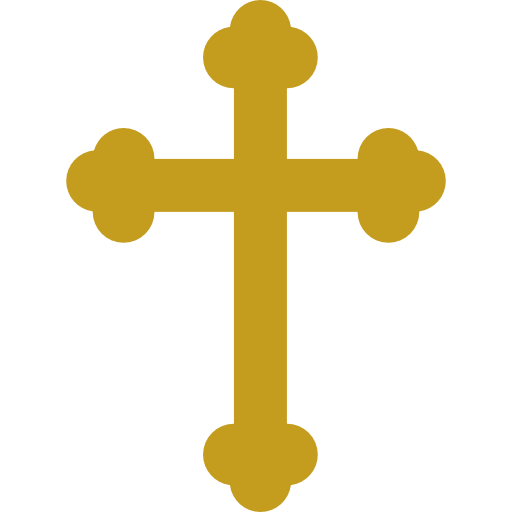
\includegraphics[scale=0.2]{assets/cross.png}\quad
  \textit{Novena a \textbf{Santo Antônio Maria Claret}}
}
\fancyfoot[RO,RE]{\thepage}

\begin{document}


\begin{center}
  {\huge Novena a Santo Antônio Maria Claret}
\end{center}

\par\noindent\rule{\textwidth}{0.4pt}

\tableofcontents
\thispagestyle{empty}

% --- Vida / Origem da Novena ---
\newpage
\section{História do Santo}
Antônio nasceu em Sallent, uma cidadezinha próxima de Barcelona, em 1807, em uma família numerosa, onde foi educado de modo profundamente cristão. Distinguiu-se logo pela sua devoção à Virgem Maria e à Eucaristia, mas, como em todas as famílias numerosas, teve que dar uma mão. Por isso, dedicou-se à atividade de tecelão, junto com seu pai. Porém, sabia bem que o seu lugar não era aquele.

\subsubsection{Encontrou seu caminho}

Em 1829, finalmente, Antônio conseguiu entrar para o Seminário de Vich. Em 1835, foi ordenado sacerdote e foi para Roma, com a ideia de partir como missionário. No início, recorreu à Propaganda Fide, o Dicastério vaticano encarregado das Missões. Porém, ali, pôde apenas fazer um curso de Exercícios espirituais, com um pregador Jesuíta, que o encaminhou à Companhia de Jesus. Assim, começou a fazer o Noviciado, mas, acometido por uma doença, teve que voltar para a Espanha, onde passou sete anos fazendo pregações por toda a Catalunha e nas Ilhas Canárias, ficando conhecido como taumaturgo. Na verdade, Antônio tinha um talento excepcional de orador e atraía a atenção pela sua vida ascética impecável: apresentava-se sempre a pé, como peregrino, com a Bíblia e o Breviário nas mãos. Em 1849, decidiu fundar uma nova Congregação de missionários, que a consagrou à Virgem, chamada “Filhos do Imaculado Coração de Maria”, que sofrerão muito durante a guerra civil espanhola, tanto que 271 deles se tornaram mártires da fé.

\subsubsection{Em missão, como pastor em Cuba}

Finalmente, seu sonho de ser missionário tornou-se realidade. Ao ser nomeado arcebispo de Santiago de Cuba – que, na época, estava sob a jurisdição da Coroa da Espanha – em 1851, partiu para a capital cubana, onde encontrou uma diocese desorganizada, devido à longa ausência de um pastor: clero reduzido e despreparado, seminário em ruínas, igrejas abandonadas. Então, arregaçou logo as mangas: convocou um Sínodo diocesano, estabeleceu a obrigação aos sacerdotes de fazer exercícios espirituais, chamou de volta os religiosos expulsos do país e, sobretudo, percorreu toda a extensão do seu território, visitando até os recantos mais recônditos. O novo Arcebispo dedicou-se à pobreza galopante, que o levou a fazer inimigos: em Holguin, foi atacado e ferido. Não obstante, em Cuba, em 1855, com a ajuda da venerável Maria Antónia Paris, fundou o ramo feminino da Congregação: as “Religiosas de Maria Imaculada” também chamadas “Missionárias Claretianas”.

\subsubsection{Retorno à Europa e últimos anos de vida}

Em 1857, a Rainha da Espanha convocou Antônio para voltar a Madrid, que teve que obedecer, para ser seu Confessor. Ligado à monarquia espanhola, seu destino mudou: em 1868, foi exilado, com a rainha, para Paris, onde continuou as suas pregações; em Roma, participou do Concílio Vaticano I, no qual defendeu a infalibilidade do Pontífice; enfim, refugiou-se no mosteiro de Fontfroide, em Narbona, na França, onde faleceu em 1870. Durante o rito de Canonização, presidido por Pio XII, em 8 de maio de 1950, o Papa destacou os seguintes aspectos da sua vida: “Era, aparentemente, modesto, mas também capacíssimo de impor respeito aos grandes terra… Entre tantas outras coisas maravilhosas, que iluminavam suavemente seus feitos, era um grande devoto da Mãe de Deus”.


% --- Orações Diárias ---
\newpage

\section{Novena a Santo Antônio Maria Claret}

\subsection{Oração Inicial} \label{oracao-inicial}

Senhor Deus nosso, que nos desígnios de vossa bondade adorável predestinastes a Santo Antônio Maria Claret para o ministério apostólico da salvação das almas e lhe acumulastes com especiais dons de graça, a fim de que fora ditado de santidade nos distintos estados da vida cristã.
Eu vos adoro e dou graças pelos tesouros de virtude que depositastes em sua alma, sobre tudo aquele espírito de caridade com que acolhia a quantos recorriam a ele em suas necessidades espirituais e temporais.

Concedei-me a graça de saber seguir seus exemplos e imitar suas virtudes, e especialmente a que venho a pedir-vos nesta novena mediante sua poderosa intercessão ante Vós.

Vós a peço também pelo coração Imaculado de Maria, de cujas glórias e misericórdia lhe fizestes apóstolo predileto. Amém. Rezar a continuação a oração do dia que corresponda:

Terminar cada dia com estas invocações e a oração final para todos os dias. Invocações para todos os dias:

\begin{enumerate}
  \item Glorioso Santo Antônio Maria, confessor e Pontífice da Igreja:
    Alcançai-nos vosso amor a Igreja santa e uma fidelidade inquebrantável a todos os seus ensinamentos e preceitos.

    Pai-nosso, Ave-Maria e Glória.
  \item Glorioso Santo Antônio Maria, apóstolo da Santíssima Virgem:
    Alcançai-nos vossa devoção a seu Imaculado Coração, e mediante ela a salvação de nossas almas.

    Pai-nosso, Ave-Maria e Glória.
  \item Glorioso Santo Antônio Maria, ilustre Fundador de Congregações religiosas:
    Alcançai-nos um ardente amor a Jesus, para seguir seus passos até o cume da perfeição cristã.

    Pai-nosso, Ave-Maria e Glória. 
\end{enumerate}

\subsection{Orações de Cada Dia}

\subsubsection{Primeiro Dia}

Inocência angelical

\textbf{Meditação:}

Considera os admiráveis exemplos de virtude que desde a mais terna infância de Santo Antônio Maria Claret.

Aprende de uns padres cristãos, modestos tecedores, que se distinguiam mais por suas virtudes cristãs que por sua fortuna.

Deles entende o santo temor de Deus, a piedade e um espírito de fé viva que lhe faz pensar com frequência na eternidade e na desgraça dos condenados.

Distingue por sua modéstia, por sua obediência e sobre tudo por sua inocência, que ele cultiva com uma terna devoção a Santíssima Virgem e a divina Eucaristia.

Em meio de seus jogos infantis sentia interiormente uma voz que lhe chamava; e obediente a ela, acudia ao templo aos pés da imagem de Maria o do Sacrário. Assim santificou sua infância e conservou intacta a inocência batismal.

\textbf{Invocação:}

 Glorioso Antonio Maria, que, provido com benções de doçura, consagraste ao Senhor vossa inocência, que depois guardaste incólume por toda a vida!

Infundi-nos amor fervente a graça de Deus, para que a guardemos zelosamente como o maior dos tesouros, e a recobremos imediatamente se alguma vez tivermos a desgraça de perde-la.

\subsubsection{Segundo Dia}
Vida de trabalho

\textbf{Meditação:}

Santo Antônio Maria foi em toda sua vida modelo perfeitíssimo do trabalho cristãmente aceitado e cumprido.

Já de menino seus pais lhe puseram no tear, para ajudar nas necessidades da casa.

Antonio se entregou aos trabalhos têxteis com todo empenho, mostrando neles extraordinárias habilidades e acompanhando o trabalho com a prática da piedade e a reza do santo Rosário.

Jovem, foi aos grandes centros fabris de Barcelona, onde com sua constante laboriosidade ganhou a confiança de todos e os primeiros postos na arte.

Seminarista, alternava a oração e o estudo.

Sacerdote, foi infatigável missionário, recorrendo a pé aos povos, pregando inumeráveis sermões, dando largas horas ao confessionário, roubando ao sono a maior parte da noite, que dedicava a oração, ao estudo, a composição de inumeráveis livros e opúsculos.

Somente por seu trabalho extraordinário e assíduo podem explicar-se as grandiosas obras e empresas que realizou em sua vida.

Para ele, o trabalho, acompanhado sempre da oração, foi alimento de sua vida espiritual, meio de apostolado, contribuição na obra redentora de Cristo. Assim deve ser para o cristão.

\textbf{Invocação:}

 Glorioso Santo Antônio Maria, que jovem artesão, soubeste fugir dos perigos do mundo, e na prática da piedade e na aplicação ao trabalho cotidiano encontraste o meio de santificar o alma e conservar puro e forte o corpo! ensinai-nos a compreender a virtude santificadora do trabalho cristãmente cumprido, e alcançai-nos a graça de que a vossa imitação consigamos santificar nossa vida na prática das obrigações de nosso estado. Amém.

\subsubsection{Terceiro Dia}
Fidelidade a vocação

\textbf{Meditação:}

Era Antonio todavia muito menino quando sentiu vivos desejos de ser sacerdote e empreendeu o estudi para preparar-se a se-lo.

Por obedecer a seu pai suspendeu por alguns anos, até que, experimentando mais forte o divino chamamento, começou no seminário de Vich a carreira eclesiástica.

Com que fidelidade a vocação divina, por superar toda classe de dificuldades, já quando seminarista, já quando sacerdote!

Com que docilidade as inspirações da graça, ao conselho de seus diretores, a vontade de seu Superior eclesiástico!

Por corresponder a ela, vai a Roma, regressa a Península, empreende as missões, vai aos povos que se lhe esperam, aceita o arcebispado e depois o cargo de confessor real. Seu espírito estava sempre prestes a escutar a voz de Deus em qualquer de suas manifestações; sua vontade, resolta a seguir a divina vontade até o heroísmo e a morte.

Assim realizou os desígnios de Deus, desígnios Providenciais para Espanha e para a Igreja. Assim foi um homem segundo o coração de Deus.

Invocação:

Glorioso Santo Antônio Maria, que apenas sentiste a vocação de Deus a um ministério mais alto e heróico, renunciaste ao lisonjeiro porvir que o mundo vos oferecia, abraçando o estado eclesiástico!

Alcançai-nos a graça de sermos sempre dóceis as celestes inspirações, para que, ainda a custa de dolorosos sacrifícios, sejamos seguir o divino chamamento e servir ao Senhor no posto em que ele quer que lhe glorifiquemos. Amém.

\subsubsection{Quarto Dia}
Vida de zelo

\textbf{Meditação:}

Santo Antônio Maria Claret é chamado o apóstolo do século XIX. E isso foi toda sua vida: de céu e apostolado.

Desde menino lhe infundiu o Senhor ardente desejo de salvar as almas, e esse céu foi crescendo toda sua vida.

Fez-se missionário apostólico e se entregou totalmente a obra das missões, recorrendo toda Catalunha, Canárias, a arquediocese de Cuba e depois a maior parte de Espana, anunciando apostolicamente a palavra de Deus em missões, exercícios e toda classe de pregação: a toda classe de pessoas, em todos os lugares, nas cidades mais populosas como nas menores aldeias. acompanhou este apostolado da palavra com o da imprensa, publicando inumeráveis livros e opúsculos, difundindo toda classe de boas leituras, fundando associações para a propaganda religiosa. e o completou com o apostolado do bom exemplo, na palavra, em todo sua porte, em toda sua vida santíssima, que transcendia a Deus e que somente buscava as almas para levarlas a Deus.

\textbf{Invocação:}

Glorioso Santo Antônio Maria, que ungido sacerdote do Senhor, não pensaste em outra coisa, nem ambicionaste senão evangelizar aos pobres e humildes e retornar a Deus aos pecadores arrependidos, renovando em vossa vida e nas pessoas as maravilhas e feitos dos apóstolos!

Alcançai-nos que, incendiados no céu das almas, nos empenhemos em levar a Deus a nossos irmãos extraviados, com a palavra, com o exemplo e com a oração, sendo assim verdadeiros testemunhem e apóstolos de Cristo. Amém.

\subsubsection{Quinto Dia}
Vida de oração

\textbf{Meditação:}

O céu apostólico de Santo Antônio Maria era fruto de seu amor a Deus e se alimentava em sua vida interior, em sua vida de oração.

Cultivou sempre a oração, tanto a mental como a vocal, dedicando-se a uma e a outra todos os dias.

Rezava diariamente as três partes do rosário, a Via-crúcis, o santo Triságio e muitas outras devoções.

Visitava diariamente o Santíssimo Sacramento.

Pelos caminhos rezava distintas devoções, e ao chegar aos povos invocava aos Santos e anjos tutelares dos mesmos.

Dedicava algumas horas diárias a oração mental, roubando ao sono da noite, dizendo que se creeria perdido o dia que houvesse abandonado a oração.

Fomentava este espírito com o recolhimento e a presença de Deus; e para ele se havia fabricado um oratório espiritual em seu coração, onde dia e noite adorava a Deus, suplicando-lhe continuamente por si e pelos demais.

Por isso o Senhor lhe favoreceu com graças extraordinárias e com comunicações sobrenaturais e deu fruto copiosíssimo a todos os seus trabalhos e empresas.

\textbf{Invocação:}

Glorioso Santo Antônio Maria, que no trato continuo com Deus pela oração transformaste toda vossa vida até não viver senão em Cristo e para Cristo, nos pensamentos, nos afetos e nas obras!

Alcançai-nos o espírito de oração, dai-nos a conhecer sua excelência e necessidade, ensinai-nos a prática da piedade cristã, para que mediante a oração aprendamos a viver cristãmente, a santificar nossas obras e com o cumprimento de nossos deveres conseguir a vida eterna. Amém.

\subsubsection{Sexto Dia}
Vida de penitência

\textbf{Meditação:}

Não é possível a vida cristã sem o espírito de penitência, nem menos a santidade sem a prática da mortificação.

Que exemplo nos dá disso Santo Antônio Maria Claret! A começou já de jovem, e lhe acompanhou toda a vida.

Três dias na semana se punha o cilício; outros três se disciplinava;

De estudante, se levantava muitas vezes da cama, exclamando:

" Senhor ! Vós em um casebre, e eu em uma cama? Jesus meu! Vós na cruz, e eu em um brando leito?" e se entregava assim a penitência.

Em sua vida de missionário, comia frugalíssimamente; não provava a carne nem o vinho; dormia muito pouco, e quando dormia era recostado em uma cadeira; Fazia sempre as viagens a pé, privando-se de todo refrigério.

Mais extraordinárias foram suas penitências quando arcebispo e quando confessor real, pelas especiais circunstancias em que se mantinha fiel a seu plano de austeridade e de privações.

E a estas mortificações voluntariamente tomadas, como não somar as que lhe vinham dos mesmos ministérios, dos elementos, da perseguição dos maus? bem pode exclamar, ao fim de sua vida, que levava em sua carne os estigmas de Jesus Cristo.

\textbf{Invocação:}

Glorioso Santo Antônio Maria, que pelo exercício constante da penitência e pela paciência admirável em sofrer toda classe de perseguições levaste impressa em vosso corpo a mortificação de Cristo, vivendo crucificado ao mundo e na carne!

Alcançai-nos o espírito de penitência com que possamos dominar as paixões, fugir dos falsos presentes do mundo e seguir a Jesus pelo caminho da cruz, até merecer os prêmios da glória. Amém.

\subsubsection{Sétimo Dia}
Espírito de humildade

\textbf{Meditação:}

Ensinam os Santos que a humildade é o fundamento da perfeição, a primeira virtude do cristão.

Sobre este fundamento tratou Santo Antônio Maria de levantar o templo de sua santidade.

Ele se entregou tão completamente a esse exercício.

Com a consideração de seu nada, com a meditação das divinas excelências, com o exame diário sobre esta virtude; sobre tudo, com o exercício constante de atos de humildade.

Por mais de vinte anos levou o exame particular sobre o exercício desta virtude. Fazer atos públicos de humildade, como beijar os pés dos outros, servir-lhes na mesa, fazer ofícios mais objetos, foi prática freqüente de toda sua vida, ainda quando arcebispo e confessor real.

Sobre tudo, sua humildade brilhou heróica no silêncio e na paz com que sofreu as mais horríveis calúnias em sua fama e em sua vida, sem sair nunca em própria defesa nem permitir que outros o fizessem.

Nem as aclamações lhe exaltavam, nem a perseguição lhe abatia; com igual modéstia e humildade nas dignidades que na obscuridade de seus ministérios apostólicos;

Tanto com os pobres e miseráveis, como desinteressado com os grandes. Buscava sempre a Deus; queria imitar a Jesus, manso e humilde de coração.

\textbf{Invocação:}

Glorioso Santo Antônio Maria, que, para seguir mais perfeitamente a Jesus, vos abraçaste com as humilhações e os desprezos, não buscando mais que a glória de Deus em tudo!

Alcançai-nos a humildade de coração, com a qualo possamos combater a soberba da vida, submeter-nos em todo a divina vontade e glorificar a Deus nesta vida para possui-lo felizmente na eterna. Amém.

\subsubsection{Oitavo Dia}
Vida Mariana.

\textbf{Meditação:}

Santo Antônio Maria teve uma verdadeira piedade filial para com a Santíssima Virgem; a amou e honrou sempre como a mãe terníssima.

De menino se alegrava em visitar suas imagens; de tecedor, rezava todos os dias as três partes do rosário; De estudante, se alistou em suas associações, para venerá-la mais fielmente; sacerdote, se consagrou como escravo seu por amor;

Missionário, pregou incansável suas Glórias e propagou as práticas de devoção e suas associações, especialmente o santo rosário e a devoção a seu Imaculado Coração, cuja devoção estabeleceu em todas as paróquias da arquediocese de Santiago.

Com que ternura filial amava ao Coração Imaculado de Maria ! e quão maternalmente pagou a Santíssima Virgem esta piedade de seu Servo!

Quantas vezes lhe livrou da morte, lhe deu vitória nas tentações e perigos, fez frutuosíssimos todos os seus ministérios!

\textbf{Invocação:}

Glorioso Santo Antônio Maria, que já desde os ternos anos escolheste a Santíssima Virgem por mãe e mestra de vossa vida espiritual, conseguindo assim chegar aos mais altos cumes da santidade!

Alcançai-nos para com ela verdadeira piedade de filhos; que conheçamos suas grandezas e excelências, que sintamos o atrativo de seu Coração maternal, para melhor conhecer, amar e servir a seu Santíssimo Filho,nosso Senhor Jesus Cristo. Amém.

\subsubsection{Nono Dia}
Vida Eucarística

\textbf{Meditação:}

O sacrário foi o lugar onde se formou a vida espiritual de Santo Antônio Maria e onde continuamente se incendiava seu amor a Deus e seu céu pelas almas.

Para isso visitava frequentíssimamente a Jesus Sacramentado, passava grande tempo meditando seu amor, celebrava fervorosamente a Santa Missa e de mil modos praticava sua devoção para com a Eucaristia.

Como desejava unir-se com Jesus ! "Eu me abraço espiritualmente com Jesus -dizia -, e neste abraço passaria toda a eternidade."

E continuava: " oh! Jesus ! quando na Santa Missa pronuncio as palavras da consagração, a substãncia do pão e do vinho desaparecem...

Pronunciai sobre mim as palavras da consagração: Consagrai-me, Jesus meu, para que eu desapareça, e sob minhas aparências viva unicamente Vós."

Como correspondeu o Senhor a este amor de seu Servo, unindo-o a si, concedendo-lhe o favor de conservar-se milagrosamente em seu interior as espécies sacramentais de uma Comunhão a outra, convertido deste modo como em um sacrário vivente!

Invocação:

Glorioso Santo Antônio Maria, amantíssimo de Jesus Hóstia, sacrário vivente da Eucaristia !

Alcançai-nos aquela vossa ardentíssima devoção a este santo mistério; que o veneremos com fé, que o recebamos com amor, que seja sempre nosso alimento espiritual na terra, para que possamos vê-lo, adorá-lo e glorifica-lo no céu. Amém.


\subsection{Oração Final} \label{oracao-final}
\versicle. \quad Rogai por nós, Santo Antônio Maria.

\response. \quad Para que sejamos dignos das promessas de Jesus Cristo.

\textbf{Oremos:} Senhor Deus, que adornastes com virtudes apostólicas a vosso bem aventurado confessor e Pontífice Antonio Maria, e por seu meio reunistes na Igreja novas famílias de clérigos e de Virgens:

Vos suplicamos nos concedais que, instruídos com seus saudáveis ensinamentos e confortados com seus exemplos, possamos felizmente chegar a Vós.

Por nosso Senhor Jesus Cristo. Amém. 

\vfill

\begin{center}
\subsection*{Fontes:}
Adaptado de: \underline{\href{https://www.vaticannews.va/pt/santo-do-dia/10/24/s--antonio-maria-claret--bispo--fundador-da-congregacao-dos-miss.html}{Vatican News}} e \underline{\href{https://www.espacojames.com.br/?cat=54&id=1418}{Espaço James - Portal Católico}}.
\end{center}


\end{document}
